\section{Vergleich der proaktiven, prädiktiven und reaktiven Methoden} \label{sec:BenchmarkVergleich}

Die unterschiedlichen Verfahren zum Umgang mit Unsicherheiten gilt es in diesem Abschnitt miteinander zu vergleichen. Bereits in den vorherigen Abschnitten wurden Ergebnisse der Verfahren für verschiedene Unsicherheitsszenarien aufgeführt. Für den Vergleich dienen die Ergebnisse der proaktiven Evaluation aus Abschnitt \ref{sec:BenchmarkErgebnisse_NaivMethoden} als Referenz, da Verspätungen ignoriert werden. Im Hinblick auf die Forschungsfrage aus Abschnitt \ref{sec:Ziele} gilt es zu überprüfen, wie sich der prädiktive und reaktive Ansatz für das \ac{mrcpsp} auf Basis von metaheuristischen Algorithmen bei der Erstellung von Zeitplänen in Bezug auf die Projektdauer bei Verspätungen verhält. 

\begin{table}[H]
\centering
\resizebox{0.90\textwidth}{!}{%
\begin{tabular}{ll|rrrr|rrrr|rrrr}
\toprule
                \textbf{Instance set n1} &  & \multicolumn{4}{c|}{Proactive Mean $\mu$} & \multicolumn{4}{c|}{Predictive Mean $\mu$} & \multicolumn{4}{c}{Reactive Mean $\mu$} \\
                 & Uncertainty $p$: &           0.00 & 0.05 & 0.10 & 0.20 &            0.00 & 0.05 & 0.10 & 0.20 &          0.00 & 0.05 & 0.10 & 0.20 \\
Solver & Iteration &                &      &      &      &                 &      &      &      &               &      &      &      \\
\midrule
RandomSolver & 500  &           6.30 & 7.15 & 7.91 & 9.39 &            6.16 & 6.97 & 7.74 & 9.21 &          6.27 & 6.61 & 6.97 & 7.74 \\
                 & 1000 &           5.51 & 6.40 & 7.18 & 8.69 &            5.43 & 6.27 & 7.04 & 8.56 &          5.64 & 6.03 & 6.40 & 7.16 \\
                 & 2500 &           4.66 & 5.54 & 6.34 & 7.84 &            4.47 & 5.28 & 6.09 & 7.54 &          4.69 & 5.08 & 5.52 & 6.37 \\
                 & 5000 &           3.82 & 4.70 & 5.52 & 7.03 &            3.90 & 4.70 & 5.48 & 6.95 &          3.73 & 4.21 & 4.66 & 5.65 \\ \hline
HillClimbing & 500  &           4.05 & 5.04 & 5.87 & 7.43 &            2.56 & 3.41 & 4.20 & 5.70 &          3.82 & 4.39 & 4.93 & 5.98 \\
                 & 1000 &           4.10 & 5.07 & 5.91 & 7.42 &            2.40 & 3.22 & 4.00 & 5.46 &          3.84 & 4.44 & 4.93 & 6.04 \\
                 & 2500 &           3.90 & 4.84 & 5.69 & 7.22 &            2.41 & 3.25 & 4.03 & 5.52 &          3.64 & 4.21 & 4.76 & 5.84 \\
                 & 5000 &           3.77 & 4.74 & 5.59 & 7.11 &            2.42 & 3.26 & 4.05 & 5.55 &          3.94 & 4.54 & 5.10 & 6.05 \\ \hline
TabuSearch & 500  &           1.80 & 2.77 & 3.60 & 5.13 &            1.60 & 2.47 & 3.27 & 4.76 &          1.77 & 2.45 & 3.17 & 4.44 \\
                 & 1000 &           1.23 & 2.24 & 3.11 & 4.64 &            1.26 & 2.12 & 2.90 & 4.38 &          1.21 & 1.96 & 2.68 & 4.00 \\
                 & 2500 &           0.86 & 1.85 & 2.71 & 4.24 &            0.86 & 1.70 & 2.49 & 4.00 &          0.98 & 1.76 & 2.53 & 3.94 \\
                 & 5000 &           0.56 & 1.54 & 2.39 & 3.92 &            0.61 & 1.46 & 2.26 & 3.75 &          0.50 & 1.36 & 2.10 & 3.64 \\ \hline
SimulatedAnnealing & 500  &           2.89 & 3.78 & 4.59 & 6.12 &            2.51 & 3.38 & 4.20 & 5.71 &          2.91 & 3.51 & 4.02 & 5.21 \\
                 & 1000 &           1.82 & 2.78 & 3.62 & 5.13 &            1.74 & 2.60 & 3.40 & 4.87 &          1.81 & 2.52 & 3.17 & 4.42 \\
                 & 2500 &           0.96 & 1.90 & 2.75 & 4.26 &            0.92 & 1.79 & 2.55 & 4.06 &          1.05 & 1.81 & 2.54 & 3.86 \\
                 & 5000 &           0.69 & 1.71 & 2.58 & 4.13 &            0.62 & 1.48 & 2.28 & 3.78 &          0.67 & 1.51 & 2.27 & 3.67 \\ \hline
GeneticAlgorithm & 500  &           2.28 & 3.15 & 3.94 & 5.47 &            2.17 & 2.99 & 3.77 & 5.25 &          2.17 & 2.78 & 3.36 & 4.52 \\
                 & 1000 &           1.04 & 1.92 & 2.74 & 4.24 &            1.09 & 1.92 & 2.70 & 4.18 &          1.15 & 1.85 & 2.50 & 3.90 \\
                 & 2500 &           0.57 & 1.48 & 2.31 & 3.84 &            0.57 & 1.42 & 2.20 & 3.67 &          0.55 & 1.39 & 2.16 & 3.56 \\
                 & 5000 &           0.46 & 1.40 & 2.24 & 3.79 &            0.43 & 1.27 & 2.05 & 3.54 &          0.49 & 1.32 & 2.10 & 3.53 \\
\bottomrule
\end{tabular}
}
\caption{Vergleich der Ergebnisse der pro-, prä- und reaktiven Verfahren für das Instanzset n1}
\source{Eigene Darstellung}
\label{tab:comparision_n1}
\end{table}

Tabelle \ref{tab:comparision_n1} fasst die Mittelwerte der Abweichungen zu den Optima der einzelnen Verfahren aus den vorherigen Abschnitten für das Instanzset n1 zusammen. Im Anhang \ref{sec:WeitereAuswertung_Vergleiche} befinden sich die Tabellen für die weiteren Benchmarks. \\

Diese Mittelwerte gilt es anschließend miteinander prozentual zu vergleichen. In Abbildung \ref{fig:evaluation_n1_heatmaps} werden in einer Heatmap-Darstellung die einzelnen Verfahren miteinander verglichen. Positive Werte stellen prozentuale Zunahmen und negative Werte prozentuale Abnahmen dar. 

\begin{figure}[H]

    \begin{subfigure}{0.497\linewidth}
        \centering
        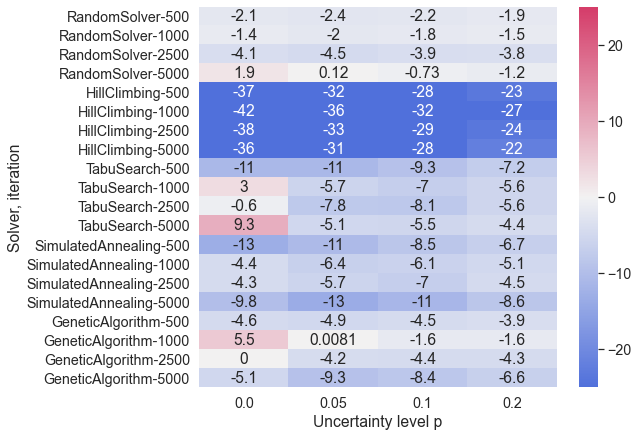
\includegraphics[width=\linewidth]{assets/img/05_Evaluation/Heatmap_n1_1.png}
        \caption{Prädiktive gegenüber proaktive Methode}
        \label{fig:evaluation_solver_n1_heatmap_1}
    \end{subfigure}
    \hfill
    \begin{subfigure}{0.497\linewidth}
        \centering
        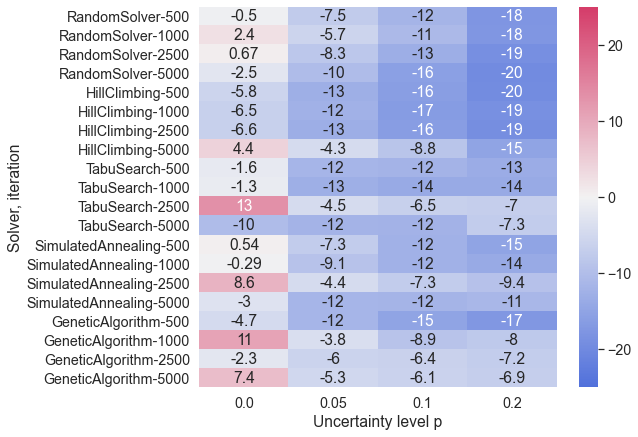
\includegraphics[width=\linewidth]{assets/img/05_Evaluation/Heatmap_n1_2.png}
        \caption{Reaktive gegenüber proaktive Methode}
        \label{fig:evaluation_solver_n1_heatmap_2}
    \end{subfigure}
    \par\bigskip 
    \begin{subfigure}{1\linewidth}
        \centering
        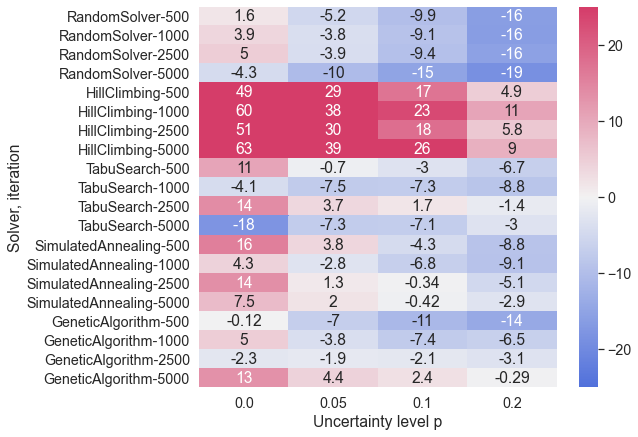
\includegraphics[width=0.5\linewidth]{assets/img/05_Evaluation/Heatmap_n1_3.png}
        \caption{Reaktive gegenüber prädiktive Methode}
        \label{fig:evaluation_solver_n1_heatmap_3}
    \end{subfigure}
    
    \caption{Heatmaps der prozentualen Abweichungen}
    \label{fig:evaluation_n1_heatmaps}
    \source{Eigene Darstellungen}
\end{figure}

Aus den Daten lässt sich erkennen, dass beim Ignorieren von Verspätungen die Abweichungen zu den Optima im Schnitt höher gegenüber der prä- und reaktiven Methode sind. Durch die Anzahl der durchlaufenden Experimente und Unsicherheitsszenarien kann bewiesen werden, dass die selektierten prädiktiven und reaktiven Verfahren einen positiven Einfluss auf die Minimierung der Verspätungen haben. \\

Innerhalb der Heatmaps lassen sich bei den Verfahren Trends über die Steigung der Unsicherheitslevel $p$ erkennen. Beim prädiktiven Ansatz über die Robustheitsoptimierung ist der beste Effekt bei $p = 0.05$ zu erkennen. Über die Erhöhung des Unsicherheitslevels sinken jedoch die prozentualen Unterschiede zum proaktiven Ansatz. Der reaktive Ansatz über das Reparieren der Zeitpläne zum Unsicherheitszeitpunkt hingegen verbessert sich über die Steigung des Unsicherheitslevels $p$, insbesondere bei einer geringen Anzahl an Iterationen bei den Basiszeitplänen. Insbesondere bei einem hohen Unsicherheitslevel ($p = 0.2$) zeigt das Verfahren deutlich höhere Unterschiede gegenüber dem proaktiven Ansatz und moderate Unterschiede gegenüber dem prädiktiven Ansatz auf. Für das \ac{mrcpsp} eignen sich prädiktive Verfahren besser für niedrigere Störungen, während reaktive Verfahren besser für komplexere Störungen geeignet sind. Dies wiederum bestätigt das, was bereits für das Basisproblem \ac{rcpsp} von \cite[vgl.][S. 405 f.]{brcic_resource_2012} über den Vergleich verschiedener Arbeiten herausgearbeitet wurde. \\

Für den direkten Vergleich von prädiktiven Verfahren gegenüber reaktiven Verfahren lassen sich jedoch Probleme feststellen, welche auf die Berechnungsdauer bezogen sind. Während prädiktive Verfahren eine feste Anzahl an Iterationen durchlaufen, werden beim reaktiven Ansatz Zeitpläne zum Unsicherheitszeitpunkt repariert, indem neue Zeitpläne gesucht werden. Hierfür wurde im Rahmen dieser Arbeit eine angepasste \acl{TS} verwendet, welche jeweils 500 Iterationen durchläuft. Dies führt dazu, dass ein weitaus höherer zeitlicher Aufwand für den reaktiven Umgang betrieben wird als gegenüber dem prädiktiven Ansatz. Basiszeitpläne, die mit einer geringen Anzahl an Iterationen gefunden wurden, profitieren von der reparierenden Tabu Suche, sodass bessere Zeitpläne gefunden werden, die bereits die Aktivitätsstörung zum Unsicherheitszeitpunkt in Betracht ziehen. Dies führt dazu, dass mit Steigung des Unsicherheitslevels die prozentualen Abweichungen bei diesen Basiszeitplänen ebenfalls steigen. Ebenfalls lassen sich bei den schwächeren Lösungsverfahren (Random Solver und Hill Climbing) in Tabelle \ref{tab:comparision_n1} deutlich geringere Differenzen zu den Basiszeitplänen feststellen. Diese Effekte gilt es bei der Interpretierung der Ergebnisse zu berücksichtigen und machen den direkten Vergleich schwieriger. \\

Bei den nachbarschaftsbasierten Algorithmen (Hill Climbing, Tabu Search und Simulated Annealing) lässt sich zudem ein weiterer Nebeneffekt innerhalb der Basiszeitpläne beim prädiktiven Ansatz erkennen. Es werden im Schnitt bessere Ergebnisse erzielt, wenn ein Algorithmus die Robustheit $\Omega$ mit berücksichtigt wird. Dies ist insbesondere in den Heatmaps aus den Abbildungen \ref{fig:evaluation_solver_n1_heatmap_1}, \ref{fig:evaluation_solver_m1_heatmap_1}, \ref{fig:evaluation_solver_m2_heatmap_1} zu erkennen. Insbesondere Hill Climbing profitiert von der Robustheitsoptimierung, sodass signifikant bessere Basiszeitpläne erzeugt wurden, welche weiterhin im Vergleich zu den Basiszeitplänen der Tabu Suche schlechter ausfallen. \\ 

Des Weiteren lässt sich in Abbildung \ref{tab:comparision_n1} erkennen, dass die Güte der Metaheuristiken auch nach Anwendung der Unsicherheitsszenarien für alle Verfahren wesentlich für die Ergebnisse sind. Ein direkter Vergleich ist somit schwierig. Im Abschnitt \ref{sec:BenchmarkErgebnisse_MetaheuristischeVerfahren} zeigte sich insbesondere der \ac{GA} als statistisch bestes der implementierten Lösungsverfahren bei der Findung von Basiszeitplänen für eine Vielzahl an Benchmark Sets. Dies und das Muster aller Lösungsvarianten ist auch nach Anwendung der Unsicherheitsszenarien zu erkennen, jedoch etwas abgeschwächter als zwischen den Basiszeitplänen. Die Wahl der Lösungsvarianten und die Anzahl der zu durchlaufenden Iterationen gilt es ebenfalls zu optimieren, um so die bestmöglichen Zeitpläne auch mit Verspätungen zu erhalten. \\

Die Intensität der Verfahren für den Umgang von Unsicherheiten hängt nicht zuletzt vom Benchmark Set ab. Während beim Benchmark Set m1 die prozentualen Abweichungen eher gering sind (vgl. Abbildung \ref{fig:evaluation_m1_heatmaps}), sind diese bei den komplexeren Sets m2 (vgl. Abbildung \ref{fig:evaluation_m2_heatmaps}), n1 (vgl. Abbildung \ref{fig:evaluation_n1_heatmaps}) und n0 (vgl. Abbildung \ref{fig:evaluation_n0_heatmaps}) stärker. 

% Welche Auswirkungenhaben präadiktive und reaktive Ansätze für das MRCPSP auf Basis von metaheuristischen Algorithmen bei der Erstellung von Zeitpläanen in Bezug auf die Projektdauer bei Verspätungen?

%%%% Die Forschungsfrage wird Mithilfe weitere Unterfragen gestützt. Welche prädiktive und reaktive Ansätze können für das MRCPSP in Kombination mit metaheuristischen Algorithmen angewandt werden? Lässt sich ein Vergleich zwischen prädiktiven und reaktiven Ansätzen auf das Ergebnis in Bezug zur Projektdauer ziehen? Welcher Einfluss haben hierbei Metaheuristiken zur Findung von \glqq guten\grqq{} Lösungen? \\